% $v_i$m:ts=4:sw=4
% Copyright (c) 2014 Casper Ti。 Vector
% Public domain。

\chapter{相关研究}

\section{高速公路关键路段挖掘相关研究}
	高速公路的关键路段挖掘问题研究较少,主要分为基于统计的研究方法和基于路网拓扑结构的研究方法。

	2006年,Jenelius等人提出了一种基于链接重要指数和现场曝光指数的路段重要性排序方法\parencite{Jenelius2006Importance},他们认为高速公路中的关键路段是结合路段发生危险概率和路段脆弱性得到的。路段脆弱性有很多定义,包括\ding{172}对一般事故的敏感度,即受事故影响的大小;\ding{173}对微小事故的敏感度,即当网络压力足够大时,哪些路段在发生小型事故后依然会对路网造成严重影响;\ding{174}可靠性,研究当处于严峻条件下路网的可操作性。同时脆弱性的使用范围也不同,有\ding{172}一条路段的脆弱性;\ding{173}一小块网络的脆弱性;\ding{174}整体网络的脆弱性。作者认为路网的脆弱性需要结合路段损毁概率和路段损毁后所造成的后果综合考虑,给出了判断路段重要性的目标函数:
	$$L(k)=\frac{{\sum\limits_i {\sum\limits_{j \ne i} {{w_{ij}}(c_{ij}^{(k)} - c_{ij}^{(0)})} } }}{{\sum\limits_i {\sum\limits_{j \ne i} {{w_{ij}}} } }} + \frac{{\sum\limits_{k \in {E^{nc}}} {\sum\limits_{i \in V_m^d} {\sum\limits_{j \ne i} {{w_{ij}}(c_{ij}^{(k)} - c_{ij}^{(0)})} } } }}{{{L^{nc}}\sum\limits_{i \in V_m^d} {\sum\limits_{j \ne i} {{w_{ij}}} } }}$$
	式中$c_{ij}^{(k)}$表示当路段或子路网集合$k$断裂时,交通网络的通行代价,$c_{ij}^{(0)}$是初始通行代价。$w_{ij}$表示$k$的重要性。该研究虽然可以度量高速公路中关键路段的重要性,但是函数局限于研究一条路段或者一个完整区域,没有考虑到多个路段、区域之间的相互影响。同时该文没有对算法效率进行优化,时间复杂度较高。

	2002年,Karlaftis等人提出了一种结合道路几何特征与事故发生概率的交通事故概率预测模型\parencite{Karlaftis2002Effects}。该研究从微观角度出发,提出了一种定量评估公路几何特征对事故发生率的影响的方法,之后给出一种基于HTBR的道路事故率预测方法。该方法解决了NB回归的一些缺陷。2016年8月,Kerner提出了一种基于微观道路信息的关键路段挖掘模型\parencite{Kerner2015The},该模型结合道路的集合形状,考虑驾驶员的视线等因素,利用路段安全性度量函数来挖掘关键路段。这些方法都是从微观角度出发,没有体现整体的网络特性。

	2016年,Yip等人基于高速公路统计学方法\parencite{YipTongji}研究高速公路路段的重要程度。该文章从高速公路拥堵情况出发,讲述了高速公路关键路段挖掘的意义,并且基于弗吉尼亚的交通管控系统,文章中使用jackson network来进行路段事故概率预测,流程如图\ref{}。通过VDOT发布的SSP数据,结合路段长度、平均行驶速度等数据,获取路段的事故概率,构建概率模型,构建jackson network预测模型来预测关键路段。

			\begin{figure}[h]
			\centering
					\begin{minipage}{0.8\linewidth}
						\centering
						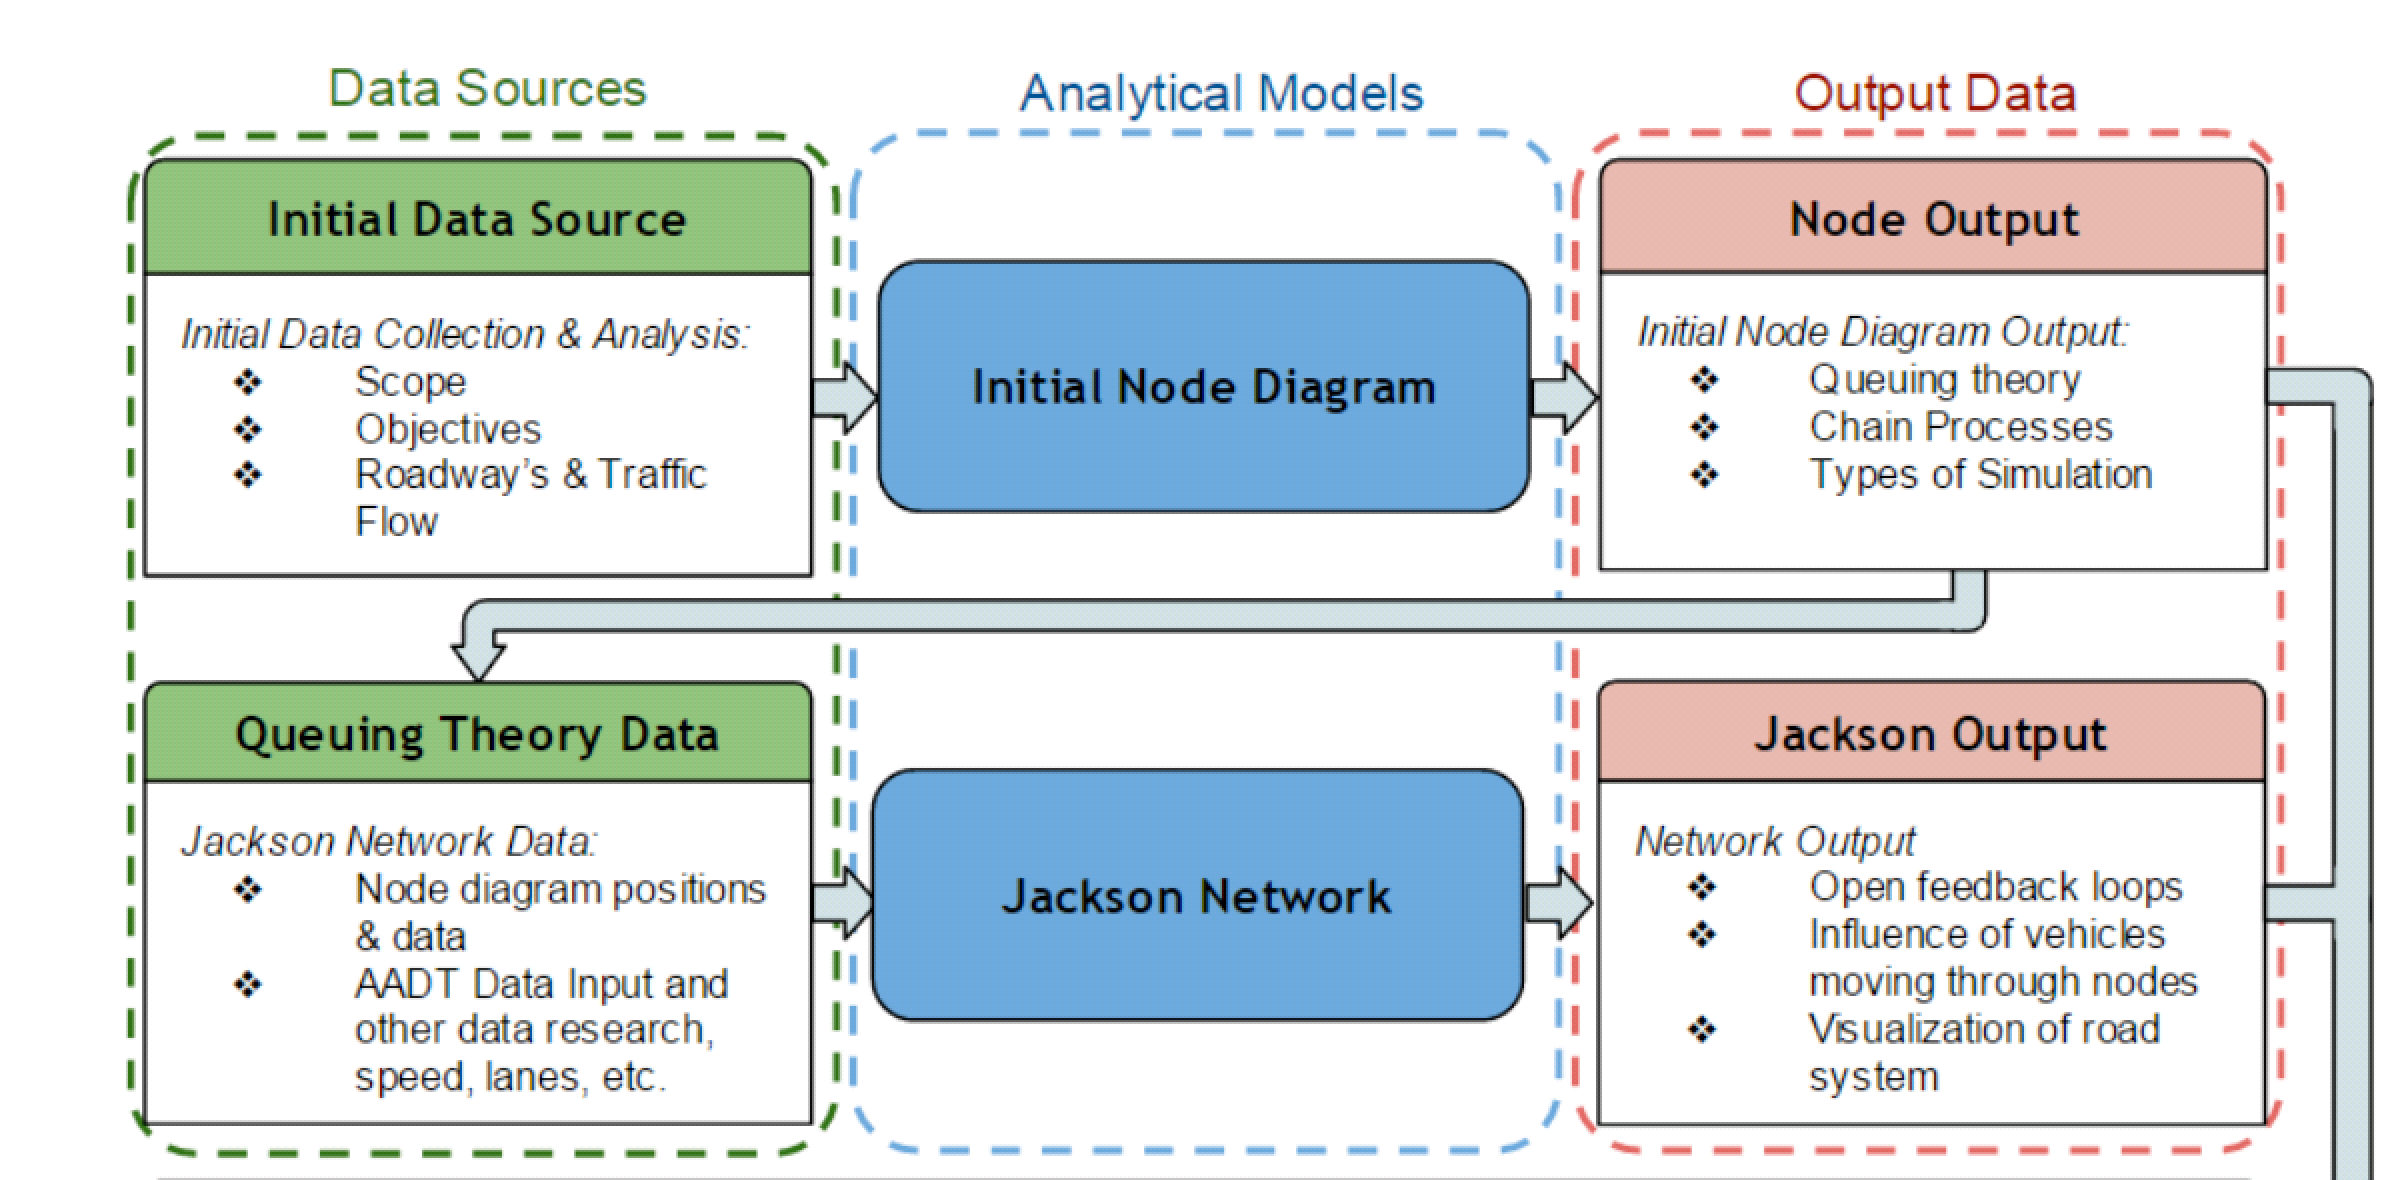
\includegraphics[width=3in]{picture/jackson_network}
						\caption{基于统计分析的关键路段识别模型}
						\label{jackson}
					\end{minipage}
			\end{figure}


	2017年,Yacine结合路段滑坡敏感性,给出了君士坦丁公路中路段的敏感性挖掘方法\parencite{Yacine2017Landslide},该方法结合路段的历史信息,通过解读航拍信息,遥感图像和实地调查,定义并研究了高速公路路段的滑坡性质。同时使用地理信息系统(GIS)为每个地理环境因素生成主题层图,从地质数据库中提取岩性单位和断层图的距离,结合数字高程模型(DEM)计算的斜坡坡度,坡度和距离,在GIS环境中对滑坡相关因素与滑坡事件之间的关系进行分析,获取易发生滑坡的路段。2014年,Ren等人基于节点的重要程度进行链接位置的优化,他们用节点的地理指标和集群特性来判定节点的重要程度,研究如何优化路段的连接方式和连接位置。这些方法从微观角度出发,通过研究节点和路段的特性来计算重要性,忽略了宏观交通流对整体网络的影响。

	2015年,Niu等人通过节点重要性评估方法研究关键节点\parencite{Niu2015Evaluation},他们提出了一种基于图论和网络理论评估公路网节点重要性的新方法,首先为每个具有GDP,里程,容量等权重的节点提出了一个效益函数,并计算出一个效益指标,表示每个节点的本地重要性;其次,为了描述整个网络的全球重要性,对节点之间的距离估计进行加权。通过地方和全球重要性的加权平均来计算每个节点的整体重要性。2011年,Song等人基于因子分析法,结合k-means算法对每个节点的重要程度进行进一步的划分\parencite{Song2011Node}。2011年,Wang等人基于节点的度、介数和交通量进行关键路段研究,同时结合C-means聚类方法进行进一步排序\parencite{Wang2011Signal}。2013年,他们又根据节点删除法来进行关键节点的识别\parencite{Wang2013Calculating},通过研究高速公路的级联失效性质,提出了基于节点失效、考虑连锁故障的交通网络节点重要性评估方法,它使用级联故障网络的拥塞状态来描述节点的重要性。2010年,Chen等人认为影响节点重要程度的因素有很多,而且它们的权值固定不变,基于这个思想,提出了一种基于Matlab聚类分析的解点重要性划分方法。

	2010年,Peeta等人提出了基于两层决策模型的关键路段挖掘方法\parencite{Peeta2010Pre},综合研究路段断裂后的连通性和路网通行效率,提出了一个度量高速公路路段重要性的模型。忽略路段之间的一阶联系,对离散函数进行求导,最终转化为背包问题进行线性时间复杂度的求解。该方法从宏观角度综合考虑了路段对整个高速公路系统的影响,但是该研究只针对桥梁,并且没有分析只考虑一阶路段影响的误差。

	现有的高速公路的关键路段研究较少,且大都是基于微观角度、基于统计学特性、基于路网结构求解,有各自的局限性。基于微观角度的研究方法虽然可以模拟真实情况下的路网状况,但是这类研究单纯的研究细节层面的高速公路网络规律,忽视了宏观层面的整体情况。基于统计学的研究方法虽然可以简单直观的根据历史先验经验,快速总结出规律,挖掘出路网的关键路段,但是这类基于经验的方法效果无法得到保证。基于网络拓扑结构虽然是研究各种复杂网络特性的经典方法,但是高速公路网络属于稀疏网络,网络复杂程度低,路网主要受到车流流量的影响。

\section{复杂网络关键路段挖掘相关研究}
	复杂网络中,关键节点的研究较多,关键路段的研究较少。因为传统的复杂网络(如社交网络)的边不具备实际的物理意义。近年来,复杂网络中,越来越多的人开始研究节点重要性排序。针对不同类型的网络,节点的重要性评价方法各不相同,且应用领域极广,研究者们从各种实际问题出发,设计出不同的方法。这些方法可以作为关键路段研究的参考。

	在交通研究中,可以对路网进行对偶拓扑,路段变成节点,节点变为边,关键路段挖掘转化为对路网中的关键节点挖掘。复杂网络关键节点研究中,主要用节点的连通性、聚类系数、空间分布、平均距离、度相关性等参数来度量节点的重要程度。通过网络的抗毁性、传播性等数据来测试网络的稳定性和完备性。其中,基于空间分布的方法在此并不适用,路段的结构比之节点更加简单,无法体现复杂网络的空间复杂性。

	
	\subsection{基于特征向量的排序方法}
	基于特征向量的关键路段挖掘方法研究路段的性质对网络的影响。累计提名方法和特征向量中心性主要用于无向网络,对于高速公路并不适用。PageRank算法和LeaderRank算法主要用于研究与识别网页重要性。在此主要介绍HITs算法。

	1999年,Kleinberg提出HITs算法\parencite{Kleinberg1999Authoritative},该算法认为网络中路段的重要性不能由单一指标确定。HITs算法定义每个节点具有两个度量值:\ding{172}权威值\ding{173}枢纽值。权威值指路段对信息的原创性,即由路段本身的价值;枢纽值是指连接该路段的邻居的价值。在一个包含n个路段的网络中,定义$a_i^t$和$b_i^t$分别路段$e_i$在t时刻的权威值和枢纽值,目标函数:
	$$L=\sum\limits_{j=1}^n a_{ji}h_j^t-1 + \sum\limits_{j=1}^n a_{ij}a_j^t$$
	式中$\sum\limits_{j=1}^n a_{ji}h_j^t-1$表示路段的权威值,$\sum\limits_{j=1}^n a_{ij}a_j^t$表示路段的枢纽值,可以看出这两个值之间相互影响。在高速公路领域。权威值是直接与路段相连的收费站的流量,枢纽值则是相邻节点向路段输入的流量。HITs方法可以结合路段特性与路段之间的相互影响,整体度量路段重要性。

	\subsection{基于路段移除和收缩的排序方法}
	2004年,李鹏翔提出一种基于节点移除和收缩的关键节点挖掘方法\parencite{lpx2004wl}。他认为路段的重要程度往往体现在该路段因为事故,被移除之后对网络的破坏性。从网络结构来说,某些关键路段移除后,整个网络有可能陷入瘫痪。李鹏翔等人用路段集被删除后,新路网中所有没有直接连线的节点对之间的最短跳数来度量路段的重要程度。用$C_i$ (k=1,2,···,u)表示路段被删除后,网络分化成的u个连通子图中第i个子图的节点数。易知此时不再连通的节点的数目为$\sum\limits_{i = 1}^u {\sum\limits_{r = i + 1}^u {{N_i}{N_r}} } $,定义路段的重要性等价于所有不再联通的节点之间最短距离之和:

	$$DSP(i)=\sum\limits_{(j,k)\in E} {{d_{jk}}}$$
	式中,$d_{jk}$为删除路段之前节点j与节点k之间的最短距离。该方法在衡量某些路段集合的重要性方面优势比较突出。但是,在更佳复杂的网络中,仅删除一个或几个路段时,路网的连通性没有遭到严重破坏,该方法的效果不明显。

	2004年,陈勇等人提出了节点生成树法\parencite{cy2004tx}。该方法认为,路段或者路段集删除后,网络的生成树的数目越少,路段越重要。2006年,Dangalchev对接近中心性进行了改进,提出了残余接近中心性方法\parencite{Dangalchev2006Residual},该方法在接近中心性方法的基础上,提出修正策略,提升短路径的影响力,易于计算和扩展。作者认为,路段的删除使得网络变得更加脆弱,通过度量脆弱程度来挖掘网络中的关键路段。定义当删除路段i之后,网络残余接近中心性为

				$$RCC(i)=\sum\limits_j {\sum\limits_{k\ne j} {\frac{1}{2^{d_{jk}(-i)}}}} $$
	其中 $d_{jk}^{(-i)}$为删除路段i后,节点j与k的最优路径的跳数。该方法在度量网络脆弱性方面上比其他方法优秀。

	\subsection{路段重要性排序方法的评价标准}
	主要分为\ding{172}使用鲁棒性和脆弱性评价网络性质评价网络性质\ding{173}使用传播动力学模型评价网络性质。

	网络科学研究的早期,网络结构简单,规模小。小规模网络结构简洁,功能简单,可以直接通过人力问卷等方式进行评价,将评价结果与算法进行比较。但是,现在社会中,网络规模迅速增长,很难得到一个客观有效的节点重要性评价指标。目前主流的评价想法是将算法得出的有序目标作为研究对象,研究这些对象对网络中的功能和结构的影响程度,断排序结果是否正确。
	\subsubsection{利用网络的脆弱性和鲁棒性}
	该方法主要研究网络中路段损毁后,对网络功能和结构的影响。影响越大路段越重要。用$k(i/n)$表示当$i/n$比例的路段被移除后,网络中巨片\parencite{Dereich2013Random}节点数目的比例。网络鲁棒性指标如下\parencite{Schneider2011Mitigation}:

				$$R=\frac{1}{n} \sum\limits_{i=1}^{n} {k(i/n)} $$
		文献\parencite{Iyer2013Attack}研究了在网络中使用几种排序方法,选出关键路段,并且移除路段后对网络最大连通性产生的影响。
	\subsubsection{用传播动力学模型评网络}
	在复杂网络研究领域中,传播研究的范围十分广泛\parencite{zt2005fz},如\ding{172}通信网络中的病毒传播\parencite{L2011Small}\ding{173}现实世界的病菌传播\ding{174}经济网络中的危机扩散\ding{175}电网中的相继故障\parencite{Peng2013Vaccination}\ding{176}社会网络中的信息传播\parencite{BrummittPNAS}等。所以,传染病模型也是在评价各种节点重要性挖掘方法的重要模型。传染病模型主要有SIR模型\parencite{Bonacich1972Factoring}和SIS模型\parencite{Kitsak2010Identification}。在 SIR 模型中,节点的传播能力与该节点的传播范围有关。在第二个模型中,使用“当节点处于稳态下时,该节点被感染的概率”来定义节点的传播能力。高速公路是一个物理路网,路段事故的传播具有时延性,事故的传播范围和传染概率对研究路段的重要性意义不大。

\section{复杂网络社群划分相关研究}

	现实中,许多情景都可以归类于复杂网络,如:人际关系网络、流行病传播网络、电子社交网络、电话网络、因特网和万维网等等。2002年 Girven和Newman引提出社群挖掘的概念。在社会 网中,社群代表了相似的人群;在生物网络中,社群表示具有相似功能的生物组织;万维网络中,社群代表具有很多相似性的文档类。近几年来,复杂网络一直属于热门研究领域,研究者分别采用自物理学、数学和计算机科
学领域的理论和技术,进行复杂网络社群划分研究。
	\subsection{基于划分的社群挖掘}
		2002年,Girvan和Newman提出了GN社群挖掘方法\parencite{Girvan2001Community},该方法采用的启发式规则,认为社群间链接的边介数应远大于社群内链接的边介数。边介数是指网络中,经过这条边的任意两点间最短路径的数量。算法通过边介数识别社群间链接,进而删除社群问链接,以自顶向下的思路建立一棵层次聚类树。该算法简单实用,适合计算小规模网络,但是同样的,该算法的缺点是计算速度过慢。2003年,Tyler等人结合统计方法,对GN算法进行了一定的改进\parencite{Tyler2003Email}。他们采用蒙特卡洛方法,近似估算出部分链接的边介数,通过牺牲精度来提高GN算法的运行效率。2010年,刘大有等人基于结构相似度来度量路段是否属于社群间链接\parencite{Di2010k},他们认为社群间链接的结构相似度应小于社群内链接的结构相似度,每次删除结构相似度最小的边,直到完全社群划分。该方法主要针对社交网络,对于交通网络并不适用。
	\subsection{基于模块性优化的社群挖掘}
		2004年,Newman和Girvan提出了一个模块性函数Q,用来刻画网络社群结构化的优劣\parencite{NewmanFast}。该算法通过不断合并两个现有的社群来进行社群划分。初始,定义社群数量,每个社群仅包含一个结点,作为候选解。每轮迭代中,选择合并后使函数Q增量最大的社群对进行合并(要求增量必须大于0)。自底向上的层次聚类,最终输出一棵层次聚类树,将使得Q最大的社群划分作为最终结果。2005年,Guimera和Amaral提出了基于模拟退火的模块性优化算法\parencite{Guimer2005Functional},该算法随机生成一个初始解,每轮迭代中,基于当前解,随机生成一个新的候选解,由模块化函数Q判断其优劣,结合模拟退火策略中的Metropolis准则,决定何时停止迭代。该算法产生新候选解的随机策略有以下几种:\ding{172}将结点移动到其他社群\ding{173}交换不同社群的结点\ding{174}分解社群\ding{175}合并社群。该算法聚类质量优秀,但是运行效率低。2006年,Newman朝将谱图理论引入模块性优化中\parencite{Newman2006Modularity}。通过将模块化函数转化成一个图拉普拉斯矩阵,优化社群划分效果。2008年,Blondel等人提出了一种新的模块性优化方法\parencite{Sanyal2006Viscous}。该方法结合了局部优化与多层次聚类技术,首先局部计算社群,之后将每个社群看作一个超级节点,再次进行合并。
	\subsection{基于标签传播的社群挖掘}

2007年,Raghavan等人提出了标签
传播算法\parencite{Raghavan2007Near},该
在初始化时为每个结点赋一个唯一标
签,每次迭代中,每个节点更新自身标签,更新策略是参照大多数邻居的标签。当所有结点的标签都不再变化时,社群挖掘结束。2009年,Leung等人将标签传播算法作为分析
大规模在线社会网的工具\parencite{Leung2009Towards},结合实际情况,研究算法的优势和限制,进而对算法进行了修正。同年,Barber等人将算法LPA等价为一
个优化问题,并给出对应的目标函数\parencite{Barber2009Detecting},设计了带约束的标签传播算法,该算法恰好就是社群划分的模块化函数Q。20lo年,Di等人发现,标签传播算法得到的社
区划分具有陷入局部最优解的倾向\parencite{Di2012Ant},提出一种多步层次贪婪算法,修正算法,每次可合并多个社群对。但是,在高速公路网络中,和节点的标签相比,流量更加重要,所以该类方法并不适用。

\subsection{基于动力学的社群挖掘}

2000年,Dongen等人提出了Markov聚类算
法\parencite{Dongen2000Graph},该算法基于Markov动力学理论,通过改变和调节马尔可夫
链,呈现出网络社群结构。2007年,在符号网络社群挖掘领域,杨博等人提出了基于Markov随机游走模型的启发式社群挖掘算法\parencite{jd2012fz},该算法认为,从任意社群出发,网络中的随机游走过程到达起始社群内结点的期望概率将大于到达起始社群外结点的期望概率。2008年,Rosvall等人提出了映射平衡算法
\parencite{Rosvall2008Maps}。该方法结合最小描述长度原理,使用信息传播扩散技术来探测网络社群结构。2011年,Morfirescu等人将复杂网络视为一个agent网络\parencite{Mor2009Opinion},每个agent拥有一个信念值,这些agent和邻居不停的进行会话,同时依据可信邻居的状态来更新自己的信念值,信念值的更新阈值不断衰减,最终达到收敛。该方法虽然已经广泛用于社群挖掘领域,但是算法普遍时间复杂度高,不符合高速公路实时性需求。

\subsection{基于仿生计算的社群挖掘}

2007年,Liu等人基于自然中蚂蚁的个体行为,提
出了一个用于探测邮件网络社群结构的蚁群聚类
算法\parencite{Liu2007Email},并且在之后结合聚类目标与群体相似度之距离的计算,作出改进。2009
年,Sadi等人采用蚁群优化技术发现网络中的
团,并将这些团视为新结点而构建一个简化网络,然
后通过传统社群挖掘算法来探测社群结构\parencite{Liu2010Finding}。2010年,刘大有等人从仿生角度出发提
出一个基于Markov随机游走的蚁群算法\parencite{Di2012Ant}。2007年,Tasgin等人提出了用于社群挖掘的遗传算法\parencite{Tasgin2007Community}。仿生网络结合了自然生物学知识,在具有客观规律的网络中十分适合。

\section{本章小结}
本章介绍了现有的高速公路关键路段挖掘方法、主流的复杂网络关键路段挖掘方法与复杂网络社群划分方法,并且分析先有方法的不足,无法很好的应用于高速公路关键路段挖掘。
			